\chapter{Coordination Protocol}
This chapter describes the protocol the client has to follow when using the TravelGood service. We use a UML state machine to illustrate the protocol. This can be seen in Fig.~\ref{fig:protocol}.

\begin{figure}[H]
\centering
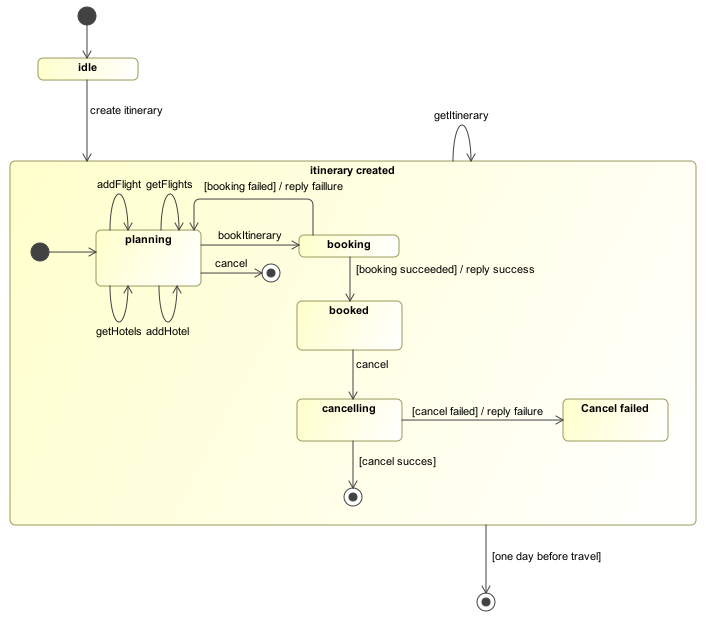
\includegraphics[width=1.0\textwidth]{Protocol}
\caption{Protocol for the web services}
\label{fig:protocol}
\end{figure}

 The protocol sits idle, until the client creates an itinerary. At this point we enter a planning state, where it is possible to search for flights and hotels, and add some of them to the itinerary. During this, the client is free to cancel, ending the protocol. If the client does not cancel, the itinerary can be booked, which is then attempted, and upon success we reach the booked state. If booking fails on some item in the itinerary, we return to the planning state. From the booked state, the client can try to cancel again and TravelGood will cancel as many items on the itinerary as possible. If all succeeds, we end the protocol, otherwise we cancel as many as we can and returned to the booked state. On the day before the travel starts, the protocol ends, if it is still running. At any time during the protocol, the client can request the current itinerary.